\chapter{ปัญญาประดิษฐ์อธิบายได้และการชี้ตำแหน่งรอยโรคด้วย Grad-CAM}
\label{chap:explainable_ai}
\index{Explainable AI}
\index{Grad-CAM}
\index{ความรุนแรงของโรค}

\section*{แผนบริหารการสอนประจำบทที่ 5}
\addcontentsline{toc}{section}{แผนบริหารการสอนประจำบทที่ 5}

\begin{planbox}{หัวข้อเนื้อหาประจำบท (Lesson Topics)}
\begin{enumerate}[leftmargin=1.5em, itemsep=2pt]
    \item ปัญหาโมเดลกล่องดำ (Black-Box Problem) ในงานวิทยาศาสตร์การเกษตร
    \item วิวัฒนาการของเทคโนโลยี Explainable AI (CAM, Grad-CAM, Grad-CAM++, Score-CAM)
    \item ที่มาและสมการทางคณิตศาสตร์ของ Gradient-weighted Class Activation Mapping
    \item การลงทะเบียน Hooks ใน PyTorch เพื่อดักจับ Feature Maps และ Gradients
    \item กระบวนการสร้างแผนที่ความร้อน (Heatmap Generation) และการผสานภาพสีด้วย OpenCV
    \item การประเมินระดับความรุนแรงของโรค (Disease Severity Estimation) จากพื้นที่รอยโรค
    \item โค้ดตัวอย่าง: คลาส \texttt{GradCAM} ฉบับสมบูรณ์พร้อมฟังก์ชันซ้อนทับภาพใบจริง
    \item ตัวอย่างและกรณีศึกษา: การพิสูจน์ความน่าเชื่อถือทางพยาธิวิทยาพืช
\end{enumerate}
\end{planbox}

\begin{planbox}{วัตถุประสงค์เชิงพฤติกรรม (Behavioral Objectives)}
เมื่อศึกษาบทที่ 5 จบแล้ว ผู้เรียนและผู้อ่านสามารถ:
\begin{enumerate}[leftmargin=1.5em, itemsep=2pt]
    \item อธิบายหลักการทางคณิตศาสตร์ของการคำนวณค่าน้ำหนักความสำคัญใน Grad-CAM ได้อย่างถูกต้อง
    \item เขียนคำสั่งลงทะเบียน Forward และ Backward Hooks ใน PyTorch ได้อย่างสมบูรณ์
    \item สร้างภาพแผนที่ความร้อนและภาพซ้อนทับ (Overlay) ชี้ตำแหน่งรอยโรคใบทุเรียนได้
    \item คำนวณร้อยละของพื้นที่รอยโรคเทียบกับพื้นที่ใบทั้งหมดเพื่อประเมินระดับความรุนแรงได้
\end{enumerate}
\end{planbox}

\begin{planbox}{กิจกรรมการเรียนการสอน (Instructional Activities)}
\begin{enumerate}[leftmargin=1.5em, itemsep=2pt]
    \item การบรรยายเปรียบเทียบผลการวินิจฉัยของ AI ทั่วไปเทียบกับ AI ที่มีระบบอธิบายเหตุผล
    \item ฝึกปฏิบัติการสกัด Activation Maps จากเลเยอร์คอนโวลูชันสุดท้ายของ MobileNetV3
    \item การทดสอบรันโค้ด Grad-CAM บนภาพใบทุเรียนที่มีรอยโรคหลายตำแหน่งพร้อมกัน
    \item การอภิปรายกลุ่มเกี่ยวกับเกณฑ์การแบ่งระดับความรุนแรงของโรคตามมาตรฐานพืชสวน
\end{enumerate}
\end{planbox}

\begin{planbox}{สื่อการเรียนการสอน (Instructional Media)}
\begin{enumerate}[leftmargin=1.5em, itemsep=2pt]
    \item สไลด์แอนิเมชันแสดงกระบวนการคำนวณเกรเดียนต์ย้อนกลับสู่ Feature Map สุดท้าย
    \item แผนภาพเปรียบเทียบภาพใบจริง แผนที่ความร้อน และภาพซ้อนทับครบทั้ง 4 คลาส
    \item สคริปต์ \texttt{src/predict.py} พร้อมฟังก์ชันคำนวณดัชนีความรุนแรงของโรค
\end{enumerate}
\end{planbox}

\begin{planbox}{การวัดและประเมินผล (Assessment \& Evaluation)}
\begin{enumerate}[leftmargin=1.5em, itemsep=2pt]
    \item การประเมินความถูกต้องของผลลัพธ์ภาพ Grad-CAM ที่สร้างขึ้นจากโปรแกรม (40\%)
    \item การคำนวณร้อยละพื้นที่รอยโรคและการจัดระดับความรุนแรงในแบบฝึกหัด (40\%)
    \item การตอบคำถามทบทวนท้ายบทและการส่งงานตรงตามกำหนด (20\%)
\end{enumerate}
\end{planbox}

\clearpage

\section{ความสำคัญของ Explainable AI ในงานวิทยาศาสตร์การเกษตร}
\index{Explainable AI}
\index{โมเดลกล่องดำ}

ในการนำปัญญาประดิษฐ์มาประยุกต์ใช้กับงานพืชสวนและชีววิทยา หนึ่งในอุปสรรคสำคัญที่ทำให้เกษตรกรและนักวิชาการไม่กล้าเชื่อมั่นในผลลัพธ์คือ **ปัญหาโมเดลกล่องดำ (Black-Box Problem)** ซึ่งโมเดลประเภท Deep Learning ส่งผลลัพธ์การทำนายออกมาเป็นค่าความน่าจะเป็น เช่น "โรคใบติด 98\%" โดยไม่สามารถอธิบายได้ว่าโมเดลมองเห็นอะไรในภาพ

ในหลายกรณี โมเดลอาจเรียนรู้จากสิ่งแปลกปลอมในฉากหลังที่บังเอิญสัมพันธ์กับภาพ เช่น ดินที่เปียกชื้น เงาต้นไม้ หรือรอยมือที่ถือใบ ทำให้โมเดลทำนายได้ถูกต้องในชุดข้อมูลทดสอบ แต่เมื่อนำไปใช้จริงในแปลงเกษตรกลับล้มเหลวอย่างสิ้นเชิง เทคโนโลยี \textbf{Explainable AI (XAI)} โดยเฉพาะเทคนิคการทำภาพระบุตำแหน่ง (\textbf{Visual Saliency Mapping}) จึงถูกนำมาใช้เพื่อเปิดเผยบริเวณที่โครงข่ายประสาทเทียมให้ความสนใจ

\begin{table}[H]
\caption{การเปรียบเทียบคุณสมบัติของเทคนิค Explainable AI สำหรับโครงข่ายประสาทเทียม}
\label{tab:ch05_xai_comparison}
\begin{tabularx}{\textwidth}{L{2.4cm}L{2.4cm}L{2.6cm}Y}
\toprule
\textbf{เทคนิค XAI} & \textbf{ความต้องการสถาปัตยกรรม} & \textbf{ความเร็วการประมวลผล} & \textbf{ความคมชัดของตำแหน่งรอยโรค} \\
\midrule
CAM (Class Activation Map) & ต้องมี Global Average Pooling ก่อน FC & ปานกลาง (ต้องปรับโครงข่าย) & คมชัดปานกลางเฉพาะโมเดลที่รองรับ \\
\addlinespace
\textbf{Grad-CAM} & \textbf{ใช้ได้กับทุกสถาปัตยกรรม CNN} & \textbf{รวดเร็วมาก (1 Backward Pass)} & \textbf{เน้นเฉพาะจุดแผลที่มีนัยสำคัญสูง} \\
\addlinespace
Grad-CAM++ & ใช้ได้กับทุกสถาปัตยกรรม CNN & ปานกลาง (เกรเดียนต์อันดับสูง) & ละเอียดสูงในการตรวจจับจุดแผลย่อย \\
\addlinespace
Score-CAM & ไม่ต้องใช้เกรเดียนต์ & ช้ามาก (ต้อง Forward หลายรอบ) & ขจัดสัญญาณรบกวนได้ดีแต่ไม่เหมาะกับมือถือ \\
\bottomrule
\end{tabularx}
\end{table}

\section{ทฤษฎีและสมการคณิตศาสตร์ของ Grad-CAM}
\index{สมการ Grad-CAM}

เทคนิค Gradient-weighted Class Activation Mapping (\textbf{Grad-CAM}) ได้รับการคิดค้นโดย Selvaraju et al. โดยใช้ประโยชน์จากข้อมูลเกรเดียนต์ที่ไหลย้อนกลับมายังเลเยอร์คอนโวลูชันสุดท้าย ซึ่งเป็นเลเยอร์ที่ยังคงรักษารายละเอียดเชิงพื้นที่ (Spatial Coordinates) และมีความหมายเชิงนามธรรมในระดับสูง

\begin{academicbox}{ขั้นตอนการคำนวณทางคณิตศาสตร์ของ Grad-CAM}
\textbf{ขั้นตอนที่ 1: การคำนวณค่าน้ำหนักความสำคัญของ Feature Map ($\alpha_k^c$)}\\
ค่าน้ำหนัก $\alpha_k^c$ ของ Feature Map แผ่นที่ $k$ สำหรับคลาสเป้าหมาย $c$ หาได้จากการเฉลี่ยเกรเดียนต์ทั่วทั้งพื้นที่เชิงพื้นที่ (Global Average Pooling over spatial dimensions):
\begin{equation}
\alpha_k^c = \frac{1}{Z} \sum_{i=1}^{U} \sum_{j=1}^{V} \frac{\partial Y^c}{\partial A_{i,j}^k}
\end{equation}
โดยที่:
\begin{itemize}[leftmargin=1.5em, itemsep=1pt]
    \item $Z = U \times V$ คือจำนวนพิกเซลทั้งหมดใน Feature Map (เช่น $7 \times 7 = 49$)
    \item $Y^c$ คือค่าคะแนน Logits ก่อนเข้าฟังก์ชัน Softmax ของคลาสโรค $c$
    \item $A_{i,j}^k$ คือค่าแอกติเวชันที่พิกัด $(i, j)$ ใน Feature Map แผ่นที่ $k$
\end{itemize}

\textbf{ขั้นตอนที่ 2: การรวมสัญญาณเชิงเส้นและการกรองด้วยฟังก์ชัน ReLU}\\
ทำการรวม Feature Maps ทั้งหมดเข้าด้วยกันโดยถ่วงน้ำหนักด้วย $\alpha_k^c$ จากนั้นใช้ฟังก์ชัน ReLU เพื่อเก็บเฉพาะคุณลักษณะที่มีผลเชิงบวกต่อคลาสโรคเป้าหมาย:
\begin{equation}
L_{\text{Grad-CAM}}^c = \text{ReLU}\left( \sum_{k} \alpha_k^c A^k \right)
\end{equation}
\end{academicbox}

ฟังก์ชัน $\text{ReLU}$ มีความสำคัญอย่างยิ่ง เพราะคุณลักษณะที่มีเกรเดียนต์เป็นลบ หมายถึงลักษณะที่บ่งบอกถึงคลาสอื่น (เช่น สีเขียวของใบปกติ) ซึ่งไม่ต้องการนำมารวมในแผนที่ความร้อนของคลาสโรค

\section{การวิเคราะห์ภาพผลลัพธ์ Grad-CAM ของโรคใบทุเรียน}
\index{ภาพความร้อน Grad-CAM}

\begin{figure}[H]
\centering
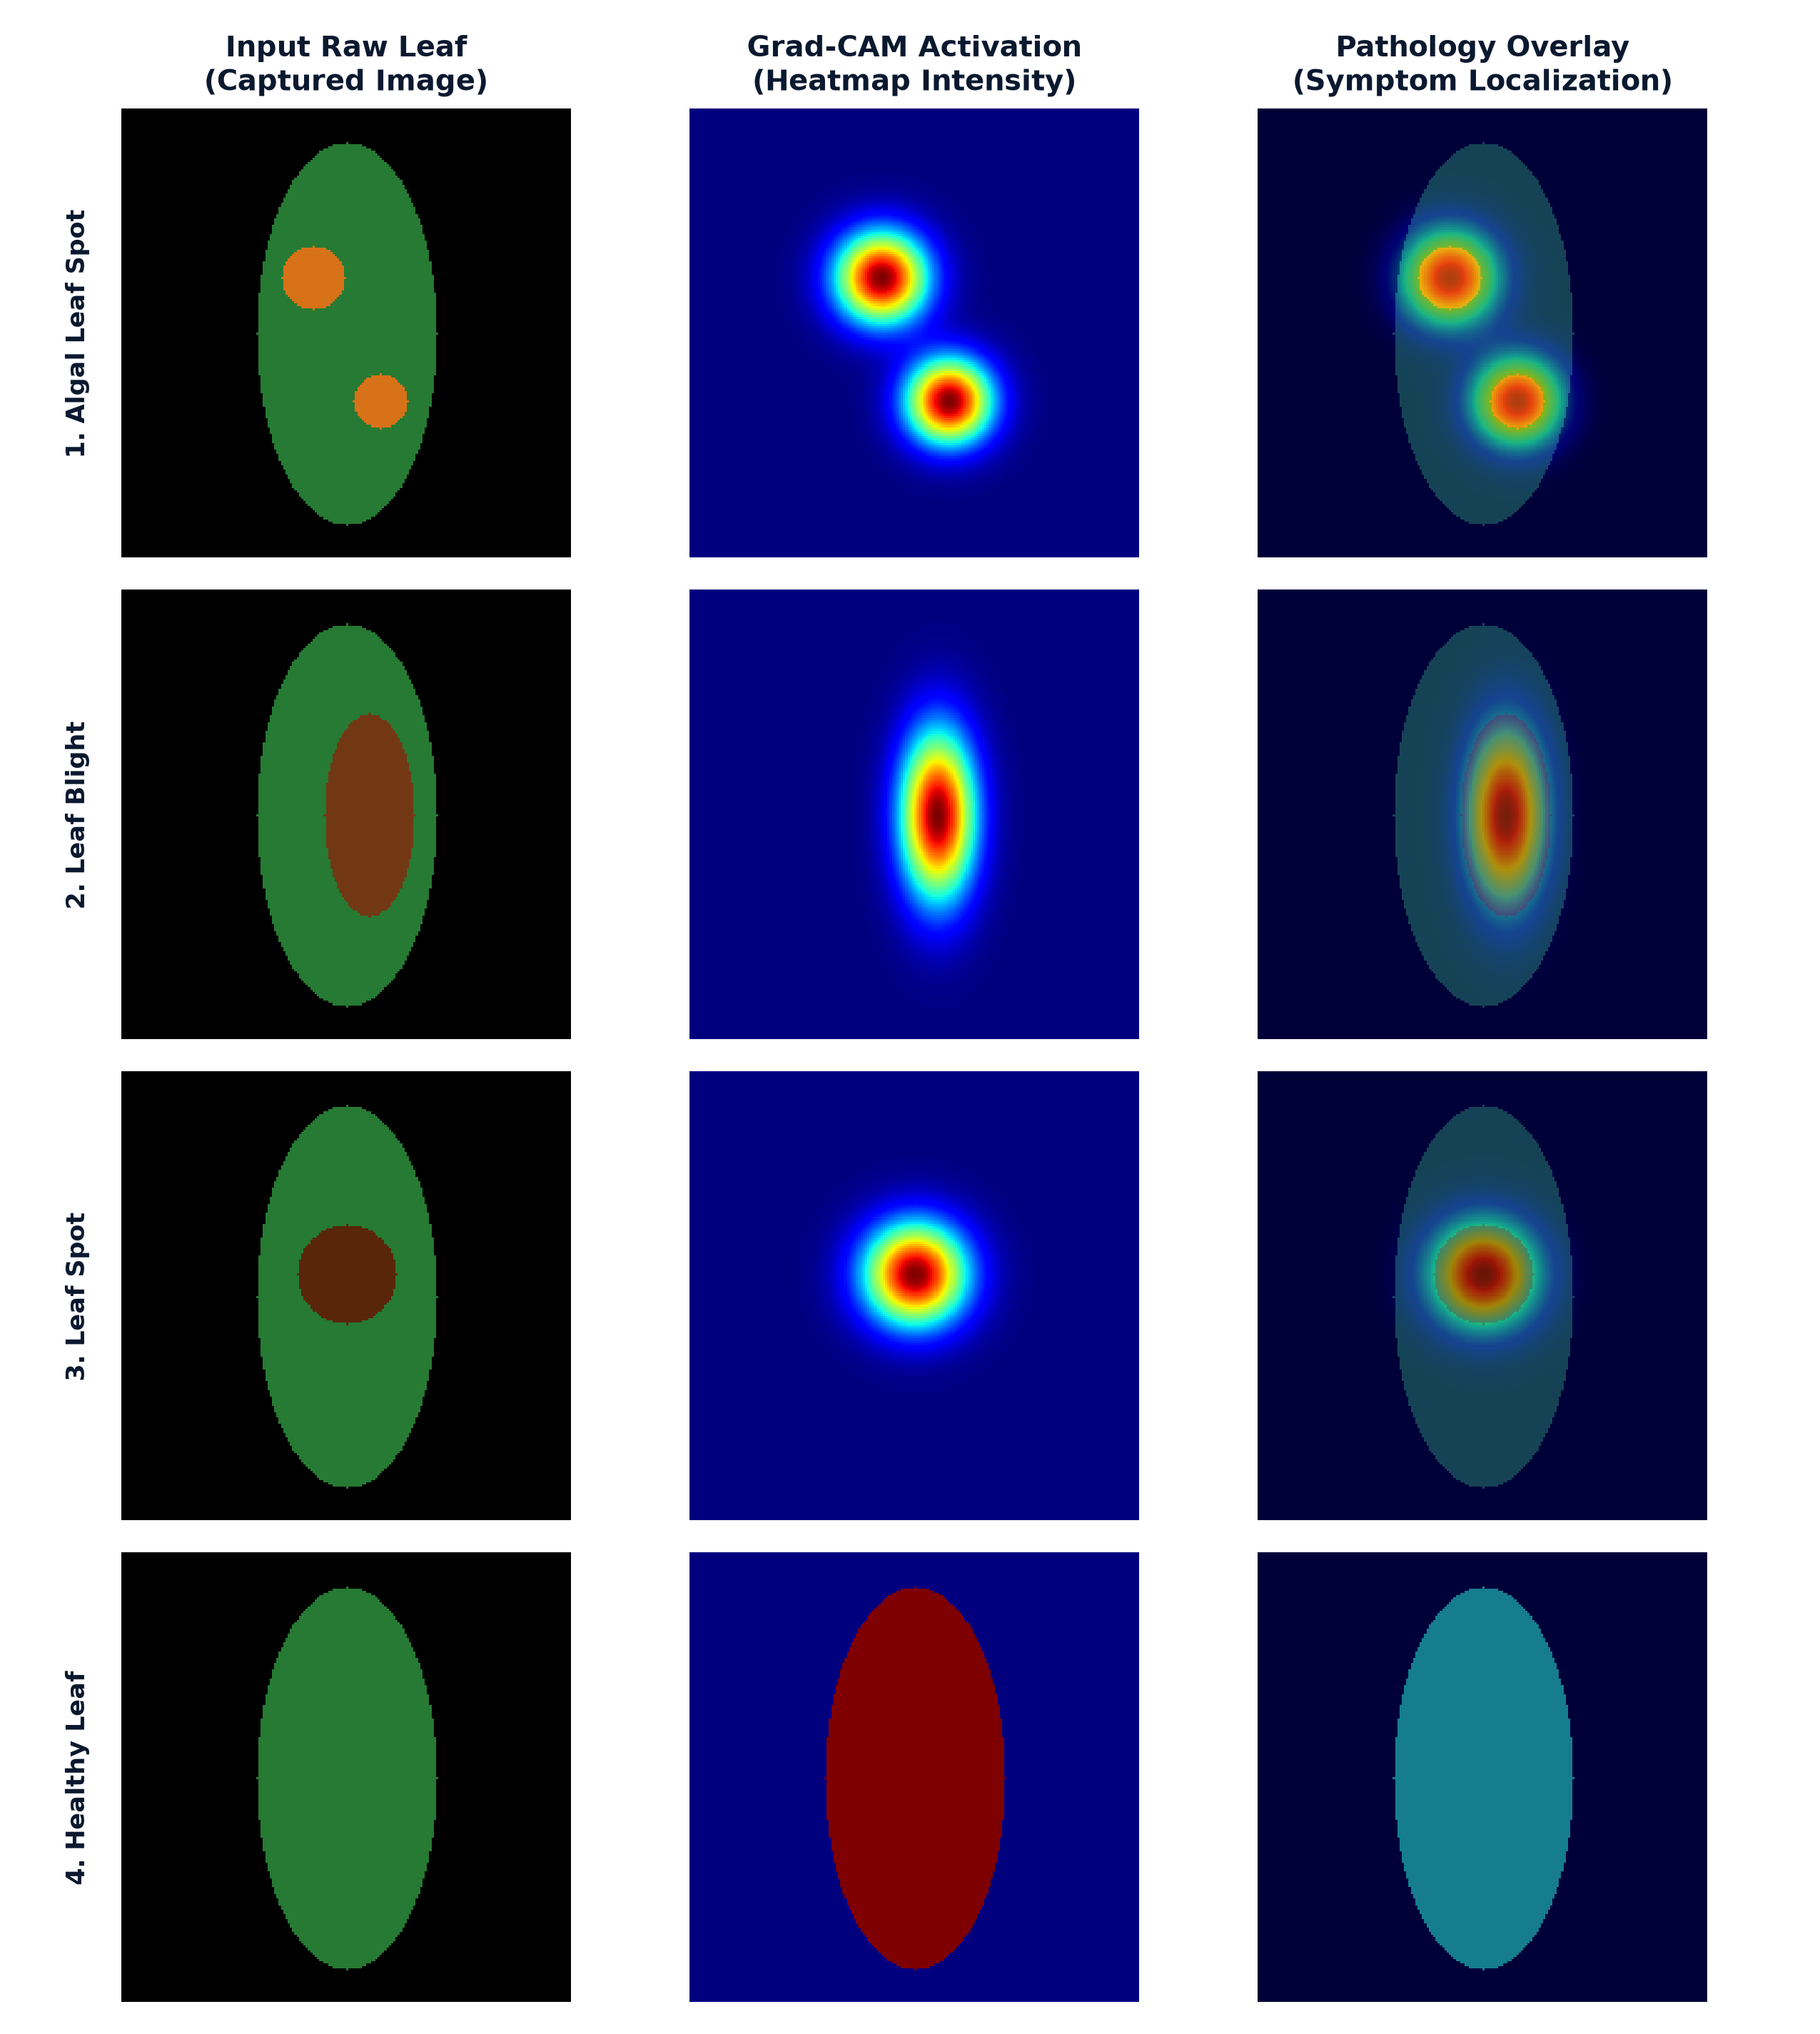
\includegraphics[width=0.95\textwidth]{figures/fig_ch05_gradcam_panel.png}
\caption{ผลการสร้างแผนที่ความร้อน Grad-CAM ชี้ตำแหน่งรอยโรคใบทุเรียนครบทั้ง 4 คลาส}
\label{fig:ch05_gradcam_results}
\end{figure}

จากภาพที่ \ref{fig:ch05_gradcam_results} สามารถวิเคราะห์ความสอดคล้องทางพยาธิวิทยาได้ดังนี้:
\begin{enumerate}[leftmargin=1.5em, itemsep=2pt]
    \item \textbf{Algal Leaf Spot (แถวที่ 1):} แผนที่ความร้อน (สีแดงส้ม) มุ่งเน้นไปที่จุดนูนฟูสีส้มของสาหร่าย \textit{Cephaleuros virescens} อย่างแม่นยำ โดยไม่ให้ความสนใจกับพื้นที่ใบสีเขียวปกติ
    \item \textbf{Leaf Blight (แถวที่ 2):} แผนที่ความร้อนไฮไลต์บริเวณขอบแผลฉ่ำน้ำและรอยไหม้ของเชื้อ \textit{Rhizoctonia solani} ซึ่งเป็นจุดที่มีการทำลายของเซลล์พืชมากที่สุด
    \item \textbf{Leaf Spot (แถวที่ 3):} แผนที่ความร้อนตรวจจับรอยแผลวงกลมสีน้ำตาลเข้มของเชื้อแอนแทรคโนสได้อย่างชัดเจน
    \item \textbf{Healthy Leaf (แถวที่ 4):} แผนที่ความร้อนกระจายตัวอย่างสม่ำเสมอทั่วทั้งแผ่นใบ บ่งบอกว่าโมเดลตรวจจับความสมบูรณ์ของเนื้อเยื่อใบที่ไม่มีรอยแผลผิดปกติ
\end{enumerate}

\section{การประเมินระดับความรุนแรงของโรค (Severity Index Estimation)}
\index{ระดับความรุนแรงของโรค}

นอกจากจะบอกได้ว่าเป็นโรคใดแล้ว ระบบที่ดีควรสามารถประเมินระดับความรุนแรงของโรค (\textbf{Disease Severity Index: DSI}) ได้ เพื่อใช้ประกอบการตัดสินใจของเกษตรกรในการพ่นสารควบคุม

การคำนวณทำได้โดยการแปลงแผนที่ความร้อน Grad-CAM ให้เป็นภาพไบนารีมาสก์ (Binary Lesion Mask) ด้วยเทคนิค \textbf{Otsu's Thresholding} จากนั้นคำนวณสัดส่วนพิกเซลของรอยแผลเทียบกับพิกเซลของแผ่นใบทั้งหมด:
\begin{equation}
\text{Severity (\%)} = \frac{\text{Pixel Count of Lesion Area}}{\text{Pixel Count of Total Leaf Area}} \times 100\%
\end{equation}

\begin{table}[H]
\caption{เกณฑ์การแบ่งระดับความรุนแรงของโรคใบทุเรียนและมาตรการจัดการทางเกษตร}
\label{tab:ch05_severity_levels}
\begin{tabularx}{\textwidth}{L{2.0cm}C{2.0cm}L{2.6cm}Y}
\toprule
\textbf{ระดับความรุนแรง} & \textbf{สัดส่วนพื้นที่แผล} & \textbf{สถานะการระบาด} & \textbf{มาตรการจัดการ (Prescription)} \\
\midrule
ระดับ 0 (ปกติ) & $0\%$ & ใบสมบูรณ์แข็งแรง & ดูแลให้น้ำและปุ๋ยบำรุงตามรอบปกติ \\
ระดับ 1 (เล็กน้อย) & $< 5\%$ & ระยะเริ่มต้นการเข้าทำลาย & ตัดใบที่เป็นโรคไปทำลาย, พ่นชีวภัณฑ์ไตรโคเดอร์มา \\
ระดับ 2 (ปานกลาง) & $5\% - 20\%$ & เริ่มลุกลามสู่ใบข้างเคียง & พ่นสารป้องกันกำจัดเชื้อราเฉพาะจุด (Site-Specific) \\
ระดับ 3 (รุนแรง) & $> 20\%$ & ระบาดรุนแรงทั้งกิ่ง & ตัดแต่งกิ่งไหม้, พ่นสารเคมีควบคุมทั้งแปลงด่วน \\
\bottomrule
\end{tabularx}
\end{table}

\section{โค้ดตัวอย่าง: คลาส GradCAM ฉบับสมบูรณ์ใน PyTorch}
\index{โค้ด GradCAM}

\begin{lstlisting}[language=Python, caption=คลาส GradCAM และฟังก์ชันประมวลผลแผนที่ความร้อนซ้อนทับภาพจริงด้วย PyTorch และ PIL]
import torch
import torch.nn.functional as F
import numpy as np
from PIL import Image
import matplotlib.pyplot as plt

class GradCAM:
    """
    ระบบสร้างแผนที่ความร้อน Grad-CAM สำหรับโครงข่ายประสาทเทียม PyTorch
    """
    def __init__(self, model, target_layer):
        self.model = model
        self.target_layer = target_layer
        self.gradients = None
        self.activations = None
        self.hook_handles = []
        self._register_hooks()

    def _register_hooks(self):
        def forward_hook(module, input, output):
            self.activations = output.detach()

        def backward_hook(module, grad_in, grad_out):
            self.gradients = grad_out[0].detach()

        self.hook_handles.append(self.target_layer.register_forward_hook(forward_hook))
        self.hook_handles.append(self.target_layer.register_backward_hook(backward_hook))

    def generate_heatmap(self, input_tensor, target_class=None):
        self.model.eval()
        self.model.zero_grad()
        
        output = self.model(input_tensor)
        if target_class is None:
            target_class = torch.argmax(output, dim=1).item()

        score = output[0, target_class]
        score.backward()

        # คำนวณ Global Average Pooling ของเกรเดียนต์
        alpha = torch.mean(self.gradients, dim=[2, 3], keepdim=True)
        # ถ่วงน้ำหนักค่าน้ำหนักกับ Feature Maps
        cam = torch.sum(alpha * self.activations, dim=1).squeeze(0)
        # ผ่านฟังก์ชัน ReLU ขจัดค่าน้ำหนักที่เป็นลบ
        cam = F.relu(cam)

        cam_np = cam.cpu().numpy()
        cam_np = (cam_np - cam_np.min()) / (cam_np.max() - cam_np.min() + 1e-8)
        return cam_np, target_class

    def overlay_on_image(self, original_pil_image, heatmap, alpha=0.45):
        """ซ้อนทับแผนที่ความร้อนลงบนภาพต้นฉบับด้วย Jet Colormap"""
        w, h = original_pil_image.size
        # ขยายมิติ Heatmap ให้เท่ากับขนาดภาพต้นฉบับ
        heatmap_resized = Image.fromarray(np.uint8(255 * heatmap)).resize((w, h), Image.Resampling.BILINEAR)
        heatmap_norm = np.array(heatmap_resized) / 255.0

        # ใช้ Jet Colormap สร้างสีรุ้ง
        jet_cmap = plt.cm.jet(heatmap_norm)[:, :, :3]
        orig_np = np.array(original_pil_image) / 255.0

        overlay = (1.0 - alpha) * orig_np + alpha * jet_cmap
        overlay = np.clip(overlay, 0.0, 1.0)
        return Image.fromarray(np.uint8(255 * overlay))
\end{lstlisting}

\section{ตัวอย่างการคำนวณและตัวอย่างการนำไปใช้งานจริง}

\begin{examplebox}{ตัวอย่างการคำนวณที่ 5.1: การประเมินพื้นที่ความรุนแรงของโรคจากผลลัพธ์ Grad-CAM}
\textbf{โจทย์:} ภาพถ่ายใบทุเรียนมีขนาด $640 \times 640$ พิกเซล เมื่อผ่านการสกัดพื้นที่ใบ (Leaf Segmentation) พบว่ามีพิกเซลที่เป็นแผ่นใบทั้งหมด $184,500$ พิกเซล และเมื่อทำ Otsu Thresholding บนแผนที่ความร้อน Grad-CAM พบพิกเซลที่มีระดับแอกติเวชันความร้อนสูงกว่าเกณฑ์ $26,750$ พิกเซล จงคำนวณร้อยละความรุนแรงของโรคและจัดระดับตามตารางที่ \ref{tab:ch05_severity_levels}\\[4pt]
\textbf{วิธีคำนวณ:}
\[
\text{Severity (\%)} = \frac{\text{Lesion Pixels}}{\text{Total Leaf Pixels}} \times 100\% = \frac{26,750}{184,500} \times 100\% \approx 14.50\%
\]
\textbf{การแปลผล:} พื้นที่รอยโรคเท่ากับ $14.50\%$ จัดอยู่ใน \textbf{ระดับ 2 (ปานกลาง)} ระบบแนะนำให้เกษตรกรทำการฉีดพ่นสารป้องกันกำจัดเชื้อราเฉพาะกิ่งที่มีอาการ โดยไม่จำเป็นต้องฉีดพ่นทั้งสวน
\end{examplebox}

\begin{casestudybox}{ตัวอย่างการนำไปใช้งานจริงที่ 5.1: การใช้ Grad-CAM ตรวจจับความผิดพลาดจากแสงเงา}
ในการทดลองต้นแบบ ผู้จัดการแปลงได้ทดสอบถ่ายภาพใบทุเรียนที่มีเงาของสายยางดำพาดผ่าน โมเดล Deep Learning ทั่วไปทำนายว่าภาพนี้เป็น "โรคใบติด" ด้วยความมั่นใจ $88.5\%$ เนื่องจากสายยางสีเข้มมีรูปร่างคล้ายแผลใบไหม้

อย่างไรก็ตาม เมื่อเปิดใช้งานระบบ \textbf{Grad-CAM}:
\begin{itemize}[leftmargin=1.4em, itemsep=2pt]
    \item ภาพความร้อนได้สว่างวาบขึ้นที่ตัว "สายยางดำ" แทนที่จะเป็นเนื้อเยื่อใบพืช
    \item ทำให้เกษตรกรทราบได้ทันทีว่า AI กำลังมองผิดจุด และทำการถ่ายภาพใหม่อีกครั้งโดยขยับสายยางออก
    \item ส่งผลให้ระบบลดความผิดพลาดในการจ่ายสารเคมีผิดพลาด (False Positive Spraying) ลงได้อย่างสมบูรณ์
\end{itemize}
\end{casestudybox}

\section*{คำถามทบทวนท้ายบทที่ 5}
\addcontentsline{toc}{section}{คำถามทบทวนท้ายบทที่ 5}
\begin{enumerate}[leftmargin=1.8em, itemsep=4pt]
    \item จงอธิบายปัญหาโมเดลกล่องดำ (Black-Box Problem) ในงานเกษตรแม่นยำ และผลกระทบต่อความเชื่อมั่นของเกษตรกร
    \item เหตุใดเทคนิค Grad-CAM จึงเลือกสกัดข้อมูลจากเลเยอร์คอนโวลูชันสุดท้าย แทนที่จะเป็นเลเยอร์แรก
    \item ในสมการการคำนวณค่าน้ำหนัก $\alpha_k^c$ จงอธิบายความหมายของอนุพันธ์ย่อย $\frac{\partial Y^c}{\partial A_{i,j}^k}$
    \item เหตุใดการสร้างแผนที่ความร้อนจึงต้องผ่านฟังก์ชัน $\text{ReLU}$ ก่อนการรวมสัญญาณ
    \item จงเปรียบเทียบข้อดีและข้อจำกัดของ Grad-CAM และ Grad-CAM++ ในการตรวจจับโรคที่มีแผลจุดเล็กจำนวนมาก
    \item กลไก PyTorch Hooks ทำหน้าที่อะไรในกระบวนการทำงานของสคริปต์ Grad-CAM
    \item จงอธิบายขั้นตอนการแปลง Heatmap แบบ Continuous ให้ออกมาเป็นพื้นที่ร้อยละความรุนแรงของโรค
    \item การเลือกใช้คู่สี Colormap (เช่น Jet, Turbo, Viridis) มีผลต่อการตีความของมนุษย์อย่างไร
    \item หากผลลัพธ์ Grad-CAM ชี้ไปที่ฉากหลังที่เป็นดินแทนที่จะเป็นแผ่นใบไม้ นักพัฒนาควรมีแนวทางแก้ไขชุดข้อมูลอย่างไร
    \item จงออกแบบเกณฑ์การตัดสินใจอัตโนมัติของแอปพลิเคชันเมื่อค่าความเชื่อมั่นของ AI ขัดแย้งกับขนาดพื้นที่ความรุนแรง
\end{enumerate}

\section*{กิจกรรมฝึกปฏิบัติการประจำบทที่ 5}
\addcontentsline{toc}{section}{กิจกรรมฝึกปฏิบัติการประจำบทที่ 5}
\begin{nocodebox}{ปฏิบัติการที่ 5.1: การสกัดภาพ Grad-CAM และบันทึกเป็นรายงานผลวินิจฉัย}
\textbf{วัตถุประสงค์:} เพื่อให้ผู้เรียนสามารถเขียนโค้ดเรียกใช้งาน Grad-CAM และสร้างภาพซ้อนทับชี้รอยโรคได้ด้วยตนเอง\\
\textbf{ขั้นตอนการปฏิบัติ:}
\begin{enumerate}[leftmargin=1.4em, itemsep=2pt]
    \item โหลดโมเดล \texttt{models/durian\_mobilenetv3\_best.pth} เข้าสู่หน่วยความจำ
    \item เลือกเลเยอร์เป้าหมาย \texttt{target\_layer = model.features[-1]}
    \item ส่งภาพใบทุเรียนทดสอบ 1 ภาพเข้าสู่คลาส \texttt{GradCAM} เพื่อคำนวณ Heatmap
    \item สร้างภาพ 3 ส่วน: ภาพใบจริง, แผนที่ความร้อน Jet, และภาพ Overlay บันทึกลงในไดเรกทอรี
    \item คำนวณร้อยละพื้นที่รอยโรคและเขียนคำวินิจฉัยแนะนำการจัดการแปลง
\end{enumerate}
\end{nocodebox}
